\chapter{Abschlussaufgabe Mean Shift}
Mean Shift ist ein parameterfreie Clusteralgorithmus. 
Mean Shift ist ein parameterfreie Clusteralgorithmus. 
Mean Shift ist ein parameterfreie Clusteralgorithmus. 
Mean Shift ist ein parameterfreie Clusteralgorithmus. 
Mean Shift ist ein parameterfreie Clusteralgorithmus. 
Mean Shift ist ein parameterfreie Clusteralgorithmus.\\
\vspace{11pt}
\begin{figure}[h]
	\centering
	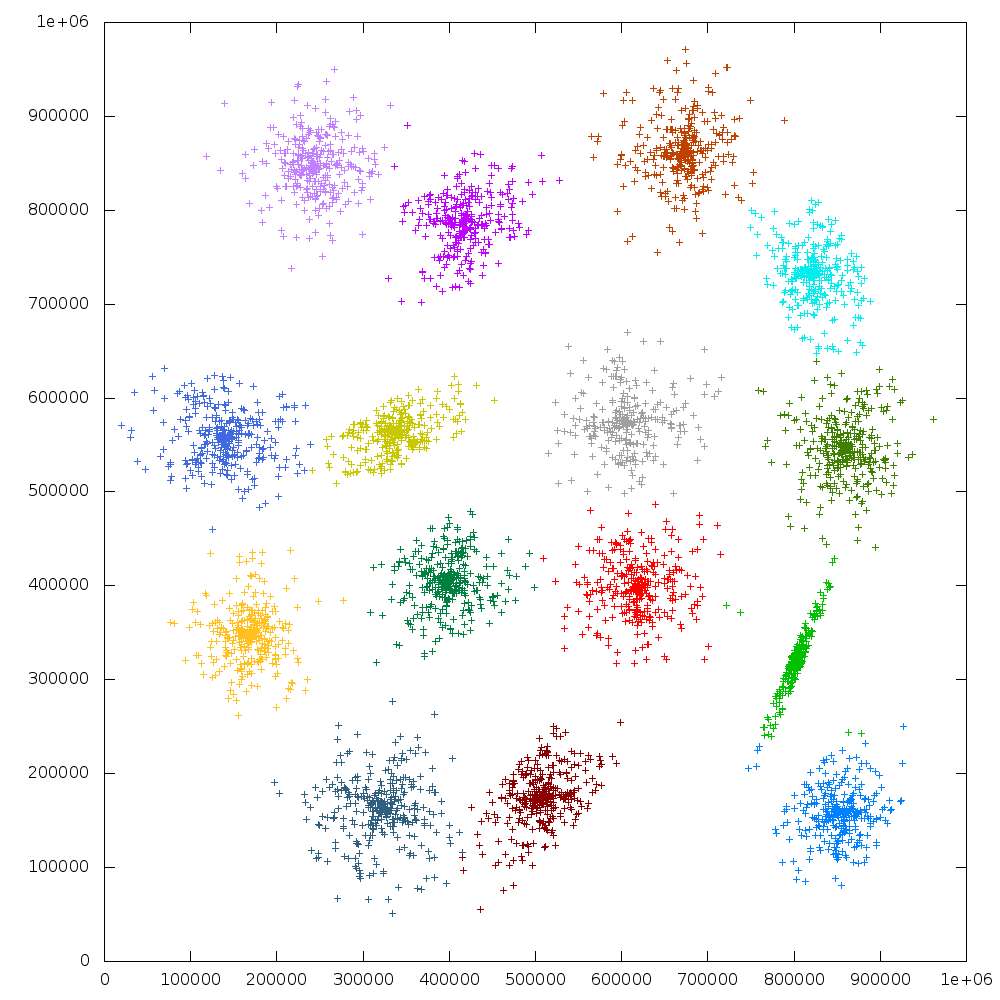
\includegraphics[scale=0.6]{../meanshift/output/pics/s1_colored.png} 
	\caption{Mean Shift S1.txt[B0]}
\end{figure}

\section{Algorithmus}
\section{Implementation}
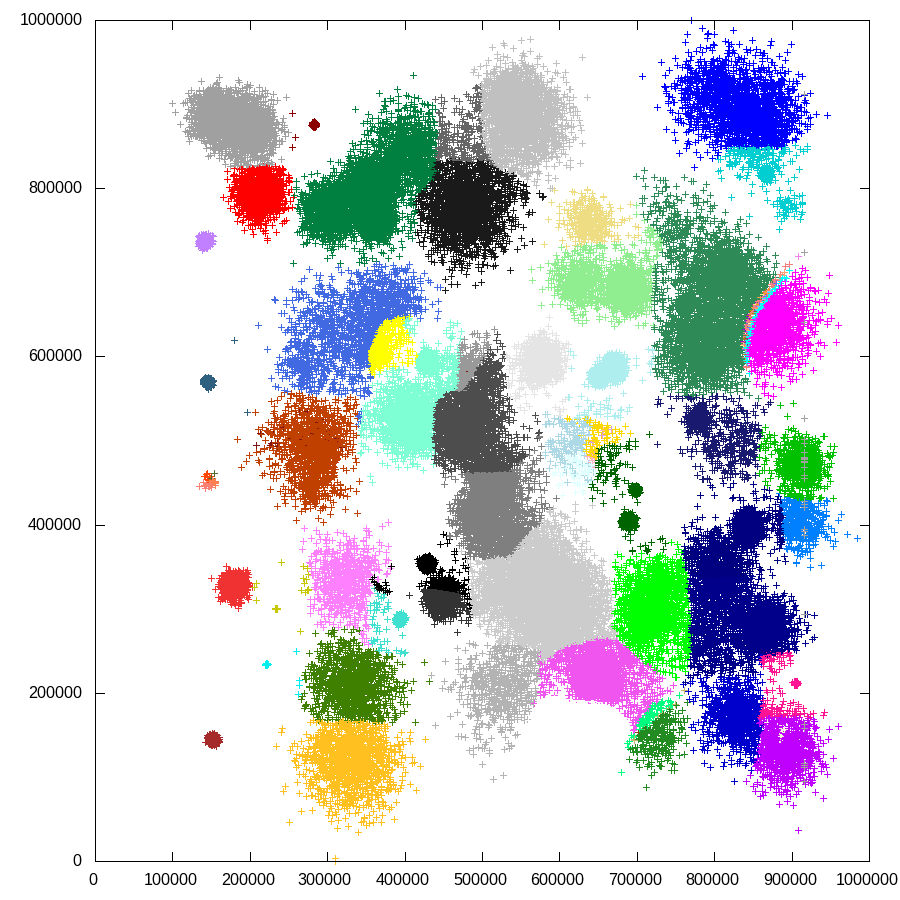
\includegraphics[scale=0.6]{../meanshift/output/pics/birch3_colored.png} 
\section{Benchmark}
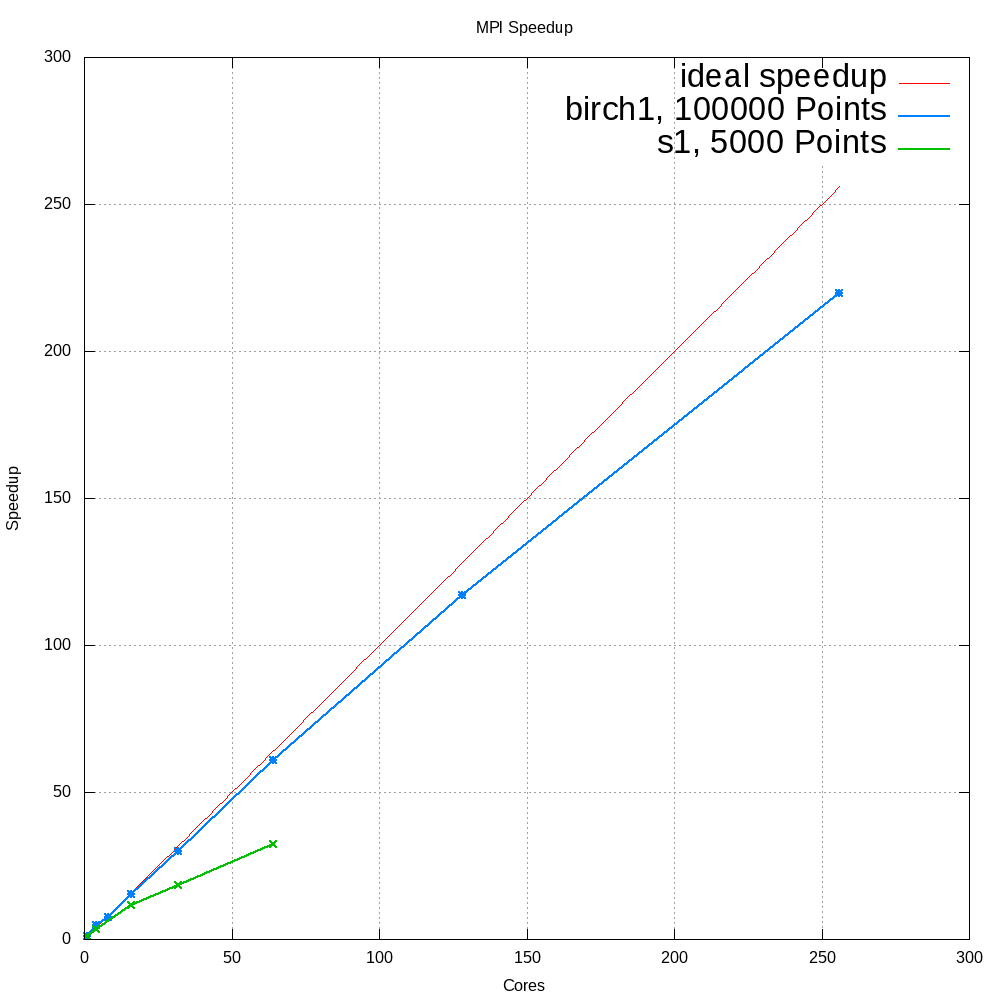
\includegraphics[scale=0.61]{../meanshift/output/pics/speedup.png} 
\newpage
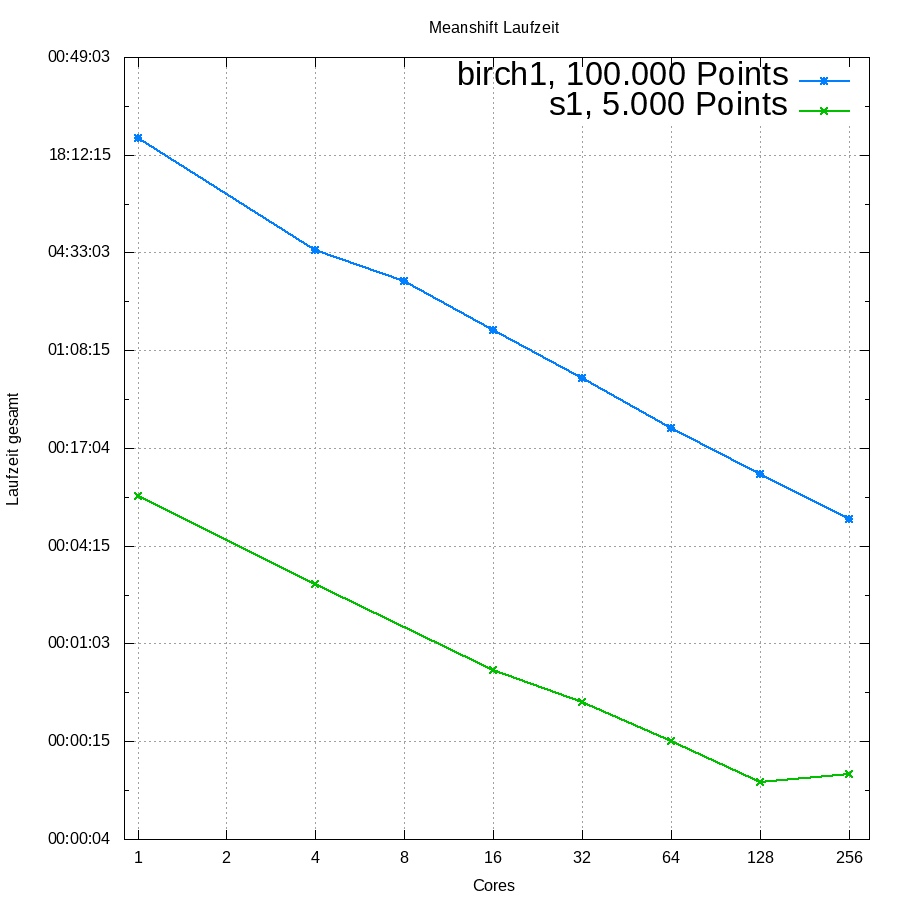
\includegraphics[scale=0.61]{../meanshift/output/pics/benchmark.png} 
\begin{thebibliography}{999}
	\bibitem [0] {} Datasets \url{http://cs.joensuu.fi/sipu/datasets/}
	\bibitem [1] {} Meanshift \url{http://homepages.inf.ed.ac.uk/rbf/CVonline/LOCAL_COPIES/TUZEL1/MeanShift.pdf}
	\bibitem [1] {} Meanshift \url{https://courses.csail.mit.edu/6.869/handouts/PAMIMeanshift.pdf}
	\newline
\end{thebibliography}
